\subsubsection{LM2596}

El regulador conmutado reductor (o \textit{Buck converter} en inglés) es un módulo que permite reducir una tensión de entrada alta a una tensión de salida menor. Esto se realiza mediante un interruptor que conmuta la corriente que atraviesa un filtro paso bajo \texttt{LC}. Además, cuenta con la virtud de que reduce la corriente de entrada, al contrario que los reguladores lineales. \cite{texasinstrumentsLM2596SIMPLESWITCHER}

En este caso, se utiliza para reducir la tensión de alimentación (tensión de $24 V$) a una tensión de $7 V$ para la entrada del \texttt{LDO}, que alimentará a los \texttt{INA226} y al \texttt{ESP8266}.

\begin{figure}[H]
    \centering
    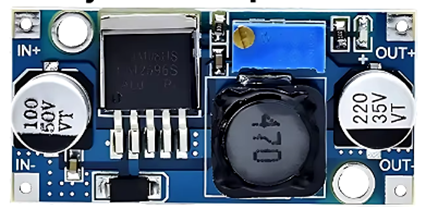
\includegraphics[width=0.5\textwidth]{images/2-hardware/componentes/LM2596.png}
    \caption{Módulo regulador reductor \texttt{LM2596}}
    \label{fig:hardware/modulos/lm2596}
\end{figure}

Con el fin de caracterizar el rendimiento, se han medido las tensiones y corrientes de entrada para dos valores de resistencia, calculando el rendimiento en ambos casos.

\begin{table}[H]
    \centering
    \begin{subtable}[t]{\textwidth}
        \centering
        \begin{tabular}{rrrrr}
            \toprule
            \multicolumn{1}{c}{Carga} & \multicolumn{1}{c}{$V_{in}$} & \multicolumn{1}{c}{$I_{in}$} & \multicolumn{1}{c}{$V_{out}$} & \multicolumn{1}{c}{$I_{out}$}\\ \midrule
            $900\ \Omega$             & $12.0045\ V$                 & $10.4268\ mA$                & $4.99920\ V$                  & $5.4825\ mA$                \\
            $100\ \Omega$             & $11.9632\ V$                 & $34.8312\ mA$                & $4.98207\ V$                  & $47.7207\ mA$                \\ \bottomrule
        \end{tabular}
        \caption{Medidas tomadas en laboratorio}
    \end{subtable}
    \\[0.5cm]
    \begin{subtable}[t]{\textwidth}
        \centering
        \begin{tabular}{rrrr}
            \toprule
            \multicolumn{1}{c}{Carga} & \multicolumn{1}{l}{$P_{in} = V_{in}\cdot I_{in}$} & \multicolumn{1}{l}{$P_{out} = V_{out}\cdot I_{out}$} & \multicolumn{1}{l}{$\eta = 100\%\cdot\frac{P_{out}}{P_{in}}$} \\ \midrule
            $900\ \Omega$             & $125. 168\ mW$                                    & $27.408\ mW$                                         & $21.897\%$                                                    \\
            $100\ \Omega$             & $416.693\ mW$                                     & $237.748\ mW$                                        & $57.056\%$                                                    \\ \bottomrule
        \end{tabular}
        \caption{Cálculos de rendimiento realizados}
    \end{subtable}
    \caption{Caracterización del rendimiento del \texttt{LM2596}}
    \label{tab:rendimiento_reductor}
\end{table}

Como se puede ver, el rendimiento incrementa con la corriente, como es natural en los reguladores conmutados, por lo que en nuestra aplicación se pueden esperar rendimientos incluso mejores.